

\section{OpticalElement: \textquotedbl{}micado\_detector\_array\textquotedbl{}%
  \label{opticalelement-micado-detector-array}%
}

\textbf{Element}: detector

\textbf{Alias}: DET

\textbf{Description}: A set of 9 H4RG detectors


\subsection{Global properties%
  \label{global-properties}%
}

\begin{quote}
\begin{alltt}
image_plane_id : 0
   temperature : -230
           dit : !OBS.dit
          ndit : !OBS.ndit
  element_name : micado_detector_array
\end{alltt}
\end{quote}


\subsection{Effects%
  \label{effects}%
}

Summary of Effects included in this optical element:

\setlength{\DUtablewidth}{\linewidth}
\begin{longtable*}[c]{|p{0.218\DUtablewidth}|p{0.199\DUtablewidth}|p{0.247\DUtablewidth}|p{0.092\DUtablewidth}|p{0.199\DUtablewidth}|}
\hline
\textbf{%
element
} & \textbf{%
name
} & \textbf{%
class
} & \textbf{%
included
} & \textbf{%
z\_orders
} \\
\hline
\endfirsthead
\hline
\textbf{%
element
} & \textbf{%
name
} & \textbf{%
class
} & \textbf{%
included
} & \textbf{%
z\_orders
} \\
\hline
\endhead
\multicolumn{5}{c}{\hfill ... continued on next page} \\
\endfoot
\endlastfoot

micado\_detector\_array
 & 
full\_detector\_array
 & 
DetectorList
 & 
False
 & 
{[}90, 290, 390, 490{]}
 \\
\hline

micado\_detector\_array
 & 
detector\_window
 & 
DetectorList
 & 
True
 & 
{[}90, 290, 390, 490{]}
 \\
\hline

micado\_detector\_array
 & 
qe\_curve
 & 
QuantumEfficiencyCurve
 & 
True
 & 
{[}113, 513{]}
 \\
\hline

micado\_detector\_array
 & 
exposure\_action
 & 
SummedExposure
 & 
True
 & 
{[}860{]}
 \\
\hline

micado\_detector\_array
 & 
dark\_current
 & 
DarkCurrent
 & 
True
 & 
{[}830{]}
 \\
\hline

micado\_detector\_array
 & 
detector\_linearity
 & 
LinearityCurve
 & 
True
 & 
{[}840{]}
 \\
\hline

micado\_detector\_array
 & 
shot\_noise
 & 
ShotNoise
 & 
True
 & 
{[}820{]}
 \\
\hline

micado\_detector\_array
 & 
readout\_noise
 & 
PoorMansHxRGReadoutNoise
 & 
True
 & 
{[}811{]}
 \\
\hline
\end{longtable*}
\label{tbl-micado-detector-array}


\subsubsection{DetectorList: \textquotedbl{}full\_detector\_array\textquotedbl{}%
  \label{detectorlist-full-detector-array}%
}

\textbf{Included by default}: \texttt{False}

\textbf{File Description}: MICADO detector array list

\textbf{Class Description}: A description of detector positions and properties

\textbf{Changes}:

\begin{itemize}
\item \{datetime.date(2017, 8, 12): '(OC) id changed to conform with spectroscopy report'\}

\item \{datetime.date(2018, 7, 26): '(OC) large gap (chips 5 and 6) reduced to 8 mm'\}

\item \{datetime.date(2018, 11, 19): '(KL) updated meta data to new format'\}

\item \{datetime.date(2019, 1, 28): '(KL) moved units into header'\}
\end{itemize}


\paragraph{Data%
  \label{data}%
}

\begin{figure}
\noindent\makebox[\linewidth][c]{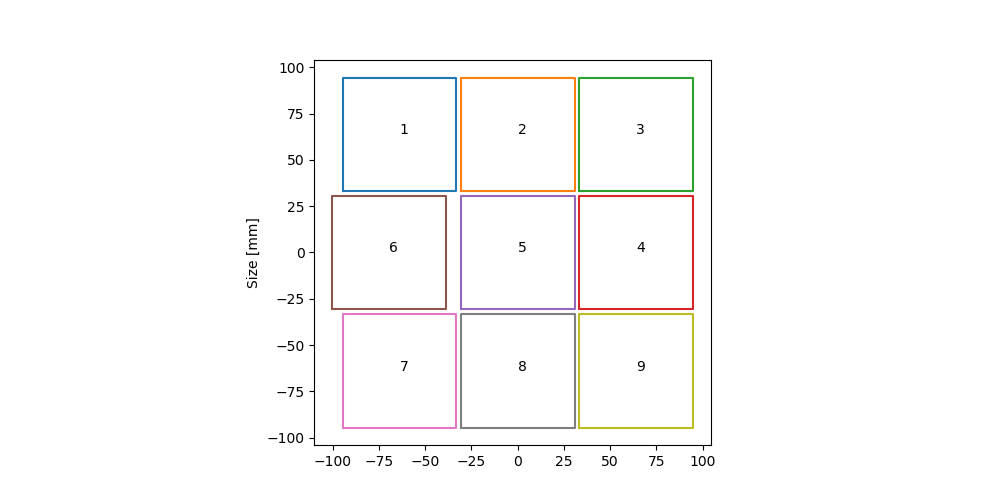
\includegraphics{full_detector_array.png}}\phantomsection\label{fig-full-detector-array}
\end{figure}

\setlength{\DUtablewidth}{\linewidth}
\begin{longtable*}[c]{|p{0.051\DUtablewidth}|p{0.086\DUtablewidth}|p{0.086\DUtablewidth}|p{0.086\DUtablewidth}|p{0.086\DUtablewidth}|p{0.075\DUtablewidth}|p{0.075\DUtablewidth}|p{0.133\DUtablewidth}|p{0.075\DUtablewidth}|p{0.063\DUtablewidth}|}
\hline
\textbf{%
id
} & \textbf{%
x\_cen
} & \textbf{%
y\_cen
} & \textbf{%
x\_size
} & \textbf{%
y\_size
} & \textbf{%
x\_len
} & \textbf{%
y\_len
} & \textbf{%
pixel\_size
} & \textbf{%
angle
} & \textbf{%
gain
} \\
\hline
\endfirsthead
\hline
\textbf{%
id
} & \textbf{%
x\_cen
} & \textbf{%
y\_cen
} & \textbf{%
x\_size
} & \textbf{%
y\_size
} & \textbf{%
x\_len
} & \textbf{%
y\_len
} & \textbf{%
pixel\_size
} & \textbf{%
angle
} & \textbf{%
gain
} \\
\hline
\endhead
\multicolumn{10}{c}{\hfill ... continued on next page} \\
\endfoot
\endlastfoot

1
 & 
-63.84
 & 
63.84
 & 
61.44
 & 
61.44
 & 
4096
 & 
4096
 & 
0.015
 & 
0.0
 & 
1.0
 \\
\hline

2
 & 
0.0
 & 
63.84
 & 
61.44
 & 
61.44
 & 
4096
 & 
4096
 & 
0.015
 & 
0.0
 & 
1.0
 \\
\hline

3
 & 
63.84
 & 
63.84
 & 
61.44
 & 
61.44
 & 
4096
 & 
4096
 & 
0.015
 & 
0.0
 & 
1.0
 \\
\hline

4
 & 
63.84
 & 
0.0
 & 
61.44
 & 
61.44
 & 
4096
 & 
4096
 & 
0.015
 & 
0.0
 & 
1.0
 \\
\hline

5
 & 
0.0
 & 
0.0
 & 
61.44
 & 
61.44
 & 
4096
 & 
4096
 & 
0.015
 & 
0.0
 & 
1.0
 \\
\hline

6
 & 
-69.44
 & 
0.0
 & 
61.44
 & 
61.44
 & 
4096
 & 
4096
 & 
0.015
 & 
0.0
 & 
1.0
 \\
\hline

7
 & 
-63.84
 & 
-63.84
 & 
61.44
 & 
61.44
 & 
4096
 & 
4096
 & 
0.015
 & 
0.0
 & 
1.0
 \\
\hline

8
 & 
0.0
 & 
-63.84
 & 
61.44
 & 
61.44
 & 
4096
 & 
4096
 & 
0.015
 & 
0.0
 & 
1.0
 \\
\hline

9
 & 
63.84
 & 
-63.84
 & 
61.44
 & 
61.44
 & 
4096
 & 
4096
 & 
0.015
 & 
0.0
 & 
1.0
 \\
\hline
\end{longtable*}
\label{tbl-full-detector-array}


\paragraph{Meta-data%
  \label{meta-data}%
}

\begin{quote}
\begin{alltt}
            filename : FPA_array_layout.dat
                name : full_detector_array
             include : False
      image_plane_id : 0
         temperature : -230
                 dit : !OBS.dit
                ndit : !OBS.ndit
        element_name : micado_detector_array
    active_detectors : all
              author : Oliver Czoske
             sources : E-MCD-FPA-572089EB.uda, ELT-TRE-MCD-56300-0011
        date_created : 2017-06-28
       date_modified : 2018-07-26
                type : detector:chip_list
          x_cen_unit : mm
          y_cen_unit : mm
            xhw_unit : mm
            yhw_unit : mm
          x_len_unit : pix
          y_len_unit : pix
        pixsize_unit : mm
          angle_unit : deg
           gain_unit : electron/adu
             z_order : [90, 290, 390, 490]
         pixel_scale : !INST.pixel_scale
 report_plot_include : True
report_table_include : True
         x_size_unit : mm
         y_size_unit : mm
\end{alltt}
\end{quote}


\subsubsection{DetectorList: \textquotedbl{}detector\_window\textquotedbl{}%
  \label{detectorlist-detector-window}%
}

\textbf{Included by default}: \texttt{True}

\textbf{File Description}:

\textbf{Class Description}: A description of detector positions and properties

\textbf{Changes}:

\begin{itemize}
\item \end{itemize}


\paragraph{Data%
  \label{id1}%
}

\begin{figure}
\noindent\makebox[\linewidth][c]{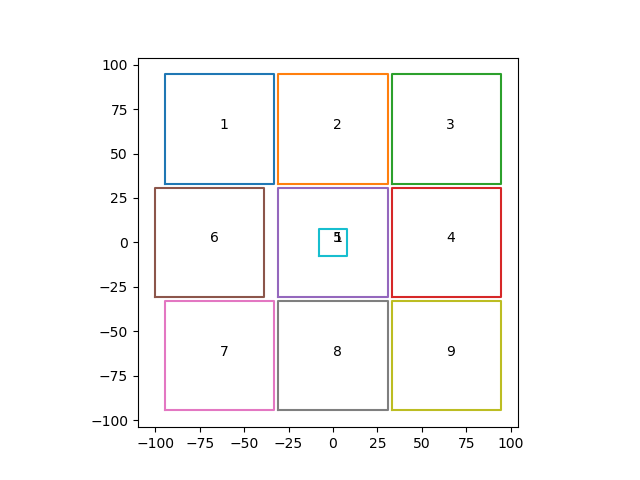
\includegraphics{detector_window.png}}\phantomsection\label{fig-detector-window}
\end{figure}

\setlength{\DUtablewidth}{\linewidth}
\begin{longtable*}[c]{|p{0.051\DUtablewidth}|p{0.133\DUtablewidth}|p{0.075\DUtablewidth}|p{0.063\DUtablewidth}|p{0.075\DUtablewidth}|p{0.075\DUtablewidth}|p{0.086\DUtablewidth}|p{0.086\DUtablewidth}|}
\hline
\textbf{%
id
} & \textbf{%
pixel\_size
} & \textbf{%
angle
} & \textbf{%
gain
} & \textbf{%
x\_cen
} & \textbf{%
y\_cen
} & \textbf{%
x\_size
} & \textbf{%
y\_size
} \\
\hline
\endfirsthead
\hline
\textbf{%
id
} & \textbf{%
pixel\_size
} & \textbf{%
angle
} & \textbf{%
gain
} & \textbf{%
x\_cen
} & \textbf{%
y\_cen
} & \textbf{%
x\_size
} & \textbf{%
y\_size
} \\
\hline
\endhead
\multicolumn{8}{c}{\hfill ... continued on next page} \\
\endfoot
\endlastfoot

1
 & 
0.015
 & 
0.0
 & 
1.0
 & 
0.0
 & 
0.0
 & 
15.36
 & 
15.36
 \\
\hline
\end{longtable*}
\label{tbl-detector-window}


\paragraph{Meta-data%
  \label{id2}%
}

\begin{quote}
\begin{alltt}
            filename : None
                name : detector_window
             include : True
      image_plane_id : 0
         temperature : -230
                 dit : !OBS.dit
                ndit : !OBS.ndit
        element_name : micado_detector_array
          x_cen_unit : mm
          y_cen_unit : mm
            xhw_unit : mm
            yhw_unit : mm
        pixsize_unit : mm
          angle_unit : deg
           gain_unit : electron/adu
             z_order : [90, 290, 390, 490]
          array_dict : \{'id': [1], 'pixsize': [0.015], 'angle': [0.0], 'gain': [1.0], 'x_cen': [0.0], 'y_cen': [0.0], 'xhw': [7.68], 'yhw': [7.68]\}
         pixel_scale : !INST.pixel_scale
    active_detectors : all
 report_plot_include : True
report_table_include : True
         x_size_unit : mm
         y_size_unit : mm
\end{alltt}
\end{quote}


\subsubsection{QuantumEfficiencyCurve: \textquotedbl{}qe\_curve\textquotedbl{}%
  \label{quantumefficiencycurve-qe-curve}%
}

\textbf{Included by default}: \texttt{True}

\textbf{File Description}: Quantum efficiency curves for each detector

\textbf{Class Description}: <no docstring>

\textbf{Changes}:

\begin{itemize}
\item \{datetime.date(2018, 11, 19): '(KL) updated meta data to new format'\}

\item \{datetime.date(2019, 8, 9): '(KL) Added action keyword to meta data'\}
\end{itemize}


\paragraph{Data%
  \label{id3}%
}


\paragraph{Meta-data%
  \label{id4}%
}

\begin{quote}
\begin{alltt}
       filename : QE_detector_H2RG.dat
           name : qe_curve
 image_plane_id : 0
    temperature : -230
            dit : !OBS.dit
           ndit : !OBS.ndit
   element_name : micado_detector_array
         author : Kieran Leschinski
        sources : Finger+ 2008 SPIE
   date_created : 2016-01-01
  date_modified : 2019-08-09
           type : detector:quantum_efficiency
         status : Design - guestimated by reading off the graph in Finger+ 2008
wavelength_unit : um
         action : transmission
        z_order : [113, 513]
        include : True
   ignore_wings : False
       wave_min : !SIM.spectral.wave_min
       wave_max : !SIM.spectral.wave_max
      wave_unit : !SIM.spectral.wave_unit
       wave_bin : !SIM.spectral.spectral_resolution
       position : -1
\end{alltt}
\end{quote}


\subsubsection{SummedExposure: \textquotedbl{}exposure\_action\textquotedbl{}%
  \label{summedexposure-exposure-action}%
}

\textbf{Included by default}: \texttt{True}

\textbf{File Description}: Summing up sky signal for all DITs and NDITs

\textbf{Class Description}: <no docstring>

\textbf{Changes}:

\begin{itemize}
\item \end{itemize}


\paragraph{Data%
  \label{id5}%
}


\paragraph{Meta-data%
  \label{id6}%
}

\begin{quote}
\begin{alltt}
      filename : None
          name : exposure_action
image_plane_id : 0
   temperature : -230
           dit : !OBS.dit
          ndit : !OBS.ndit
  element_name : micado_detector_array
       z_order : [860]
       include : True
\end{alltt}
\end{quote}


\subsubsection{DarkCurrent: \textquotedbl{}dark\_current\textquotedbl{}%
  \label{darkcurrent-dark-current}%
}

\textbf{Included by default}: \texttt{True}

\textbf{File Description}: MICADO dark current

\textbf{Class Description}: required: dit, ndit, value

\textbf{Changes}:

\begin{itemize}
\item \end{itemize}


\paragraph{Data%
  \label{id7}%
}


\paragraph{Meta-data%
  \label{id8}%
}

\begin{quote}
\begin{alltt}
      filename : None
          name : dark_current
image_plane_id : 0
   temperature : -230
           dit : !OBS.dit
          ndit : !OBS.ndit
  element_name : micado_detector_array
         value : 0.1
       z_order : [830]
       include : True
\end{alltt}
\end{quote}


\subsubsection{LinearityCurve: \textquotedbl{}detector\_linearity\textquotedbl{}%
  \label{linearitycurve-detector-linearity}%
}

\textbf{Included by default}: \texttt{True}

\textbf{File Description}: Linearity characteristics of H4RG chips

\textbf{Class Description}: <no docstring>

\textbf{Changes}:

\begin{itemize}
\item 2018-11-19 (KL) updated meta data to new format

\item 2019-08-14 (KL) replaced long 1000000000 with 1e99
\end{itemize}


\paragraph{Data%
  \label{id9}%
}


\paragraph{Meta-data%
  \label{id10}%
}

\begin{quote}
\begin{alltt}
      filename : FPA_linearity.dat
          name : detector_linearity
image_plane_id : 0
   temperature : -230
           dit : !OBS.dit
          ndit : !OBS.ndit
  element_name : micado_detector_array
        author : Kieran Leschinski
       sources : Ingraham+ 2014 - Gemini Calibrations II for H2RG
  date_created : 2016-01-01
 date_modified : 2018-11-19
          type : detector:linearity
        status : Design - approximated from the H2RG
 incident_unit : ph
 measured_unit : ph
       z_order : [840]
       include : True
\end{alltt}
\end{quote}


\subsubsection{ShotNoise: \textquotedbl{}shot\_noise\textquotedbl{}%
  \label{shotnoise-shot-noise}%
}

\textbf{Included by default}: \texttt{True}

\textbf{File Description}: apply poisson shot noise to images

\textbf{Class Description}: <no docstring>

\textbf{Changes}:

\begin{itemize}
\item \end{itemize}


\paragraph{Data%
  \label{id11}%
}


\paragraph{Meta-data%
  \label{id12}%
}

\begin{quote}
\begin{alltt}
      filename : None
          name : shot_noise
image_plane_id : 0
   temperature : -230
           dit : !OBS.dit
          ndit : !OBS.ndit
  element_name : micado_detector_array
       z_order : [820]
       include : True
   random_seed : !SIM.random.seed
\end{alltt}
\end{quote}


\subsubsection{PoorMansHxRGReadoutNoise: \textquotedbl{}readout\_noise\textquotedbl{}%
  \label{poormanshxrgreadoutnoise-readout-noise}%
}

\textbf{Included by default}: \texttt{True}

\textbf{File Description}: Readout noise frames

\textbf{Class Description}: <no docstring>

\textbf{Changes}:

\begin{itemize}
\item \end{itemize}


\paragraph{Data%
  \label{id13}%
}


\paragraph{Meta-data%
  \label{id14}%
}

\begin{quote}
\begin{alltt}
         filename : None
             name : readout_noise
   image_plane_id : 0
      temperature : -230
              dit : !OBS.dit
             ndit : !OBS.ndit
     element_name : micado_detector_array
        noise_std : 12
       n_channels : 64
          z_order : [811]
          include : True
pedestal_fraction : 0.3
    read_fraction : 0.4
    line_fraction : 0.25
 channel_fraction : 0.05
      random_seed : !SIM.random.seed
\end{alltt}
\end{quote}
